\documentclass[11pt, oneside]{article}   	% use "amsart" instead of "article" for AMSLaTeX format
\usepackage{geometry}                		% See geometry.pdf to learn the layout options. There are lots.
\geometry{letterpaper}                   		% ... or a4paper or a5paper or ... 
%\geometry{landscape}                		% Activate for for rotated page geometry
%\usepackage[parfill]{parskip}    		% Activate to begin paragraphs with an empty line rather than an indent
\usepackage{graphicx}				% Use pdf, png, jpg, or eps§ with pdflatex; use eps in DVI mode
								% TeX will automatically convert eps --> pdf in pdflatex		
\usepackage{amssymb}
\usepackage{amsmath}
\usepackage{parskip}
\usepackage{color}
\usepackage{hyperref}

\title{Surface integrals}
%\author{The Author}
%\section{}
%\subsection*{}
\date{}							% Activate to display a given date or no date

\graphicspath{{/Users/telliott_admin/Dropbox/Tex/png/}}
% \begin{center} 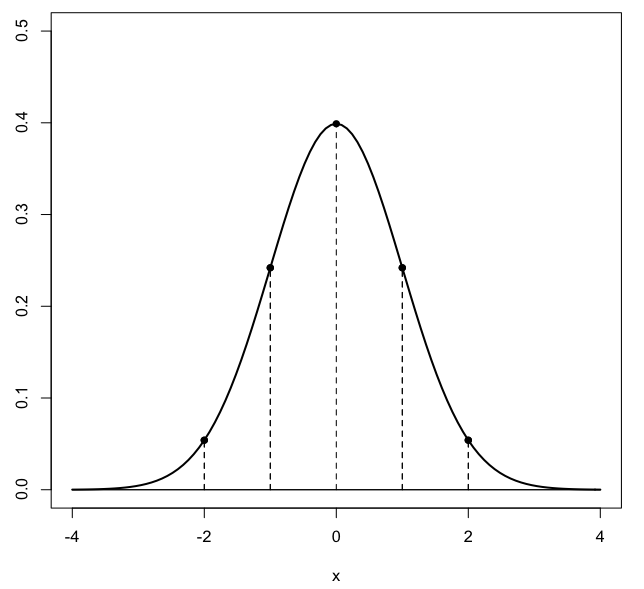
\includegraphics [scale=0.4] {gauss3.png} \end{center}
\begin{document}
\maketitle
\Large
I always have a hard time remembering how to work with surface integrals.  Let's try again.  

One helpful thing is that line integrals seem pretty straightforward to set up, though they are often an arithmetic mess.

The small element of the path is $ds$ so by Pythagoras we get 
\[ ds^2 = dx^2 + dy^2 \] 
and then a little rearrangement gives:
\[ ds^2 = \ [ \ 1 + (\frac{dy}{dx})^2 \ ] \ dx^2 \] 
\[ ds = \ [ \ \sqrt{1 + [f'(x)]^2} \ ] \ dx \]

The area element for surfaces is almost exactly the same:
\[ dS =  \sqrt{(1 + f_x)^2 + (f_y)^2} \  \cdot \ dA \]
So let's just remember the surface area element $dS$ as an extension of $ds$ to 3 dimensions.

\subsection*{sphere}
With just this formula we can calculate something like the surface area of a sphere.  Write
\[ x^2 + y^2 + z^2 = a^2 \]
where $a$ is the constant radius.  Then
\[ z = f(x,y) = \sqrt{a^2 - x^2 - y^2} \]
\[ f_x = \frac{1}{2} \ \frac{-2x}{\sqrt{a^2 - x^2 - y^2}} = -\frac{x}{z} \]
or by implicit differentiation:
\[ z^2 = a^2 - x^2 - y^2 \]
\[ 2 z \ dz = - 2 x \ dx \]
and then we get the same thing as before.  Similarly $f_y = -y/z$.

Then use the formula.  Plugging in $f_x$ and $f_y$:
\[ dS = \ [ \ \sqrt{(\frac{x}{z})^2 + (\frac{y}{z})^2 + 1} \  ] \ dA \]
\[ = \frac{1}{z}  \ [ \ \sqrt{(x^2 + y^2 + z^2} \  ] \ dA \]
\[ dS = \frac{a}{z} \ dA \]

We want to set up $\int dS$, but it's pretty ugly in $x,y$.  We get
\[ \int_{-a}^a \int_{-\sqrt{a^2-x^2}}^{\sqrt{a^2-x^2}} \frac{a}{\sqrt{a^2 - x^2 -y^2}} \ dy \ dx \]
The inner integral is essentially:
\[ \int \frac{1}{\sqrt{c^2 -y^2}} \ dy \]
for the constant $c^2 = a^2 - x^2$, and we don't have $y$ so we need to do a trig substitution.  This comes out to be
\[ \sin^{-1} \frac{y}{c} \]
evaluated between $-c$ and $c$.  
\[ \sin^{-1} \frac{y}{c} \  \bigg |_{-c}^c = \frac{\pi}{2} - (- \frac{\pi}{2}) = \pi  \]
The outer integral is then
\[ \int_{-a}^a \pi a \ dx = 2 \pi a^2 \]

It is much nicer to switch to $r,\theta$.  We do this to check ourselves. Let
\[ x^2 + y^2 = r^2 \]
\[ z^2 = a^2 - x^2 - y^2 = a^2 - r^2 \]
\[ \int dS = \int_0^{2 \pi} \int_0^a  \frac{a}{\sqrt{a^2 - r^2}} \ r \ dr \ d \theta \]

The inner integral is essentially $1/\sqrt{u} \ du$
\[ \int \frac{1}{\sqrt{a^2 - r^2}} \ r \ dr = -\sqrt{a^2 - r^2}  \]
so we obtain
\[ a \ [ \ -\sqrt{a^2 - r^2} \ ] \ \bigg |_0^a = a^2 \]
which is zero at the upper bound and $-a^2$ at the lower bound.  Subtracting, we obtain $a^2$, and with the outer integral, the whole thing is $2 \pi a^2$.

We are a factor of $2$ off from the known result using both methods, and realize that when we wrote 
\[ z = f(x,y) = \sqrt{a^2 - x^2 - y^2} \]
we were only looking at the upper hemisphere, so a factor of $2$ is missing.

\subsection*{paraboloid}
Let's do the paraboloid as well.  We can write the equation as
\[ z =  c - x^2 - y^2 \]
This one opens down, and the vertex is at $z = c$.

Suppose the sign of the $c$ term is positive and we want the area above the $xy$-plane.  In the plane, $z = 0$ so
\[ x^2 + y^2 = r^2 = c \]
The radius of the circle in the plane is $\sqrt{c}$.  That will be the upper bound of the radial integral in polar coordinates.

Recall our formula
\[ dS = \ [ \ \sqrt{(f_x)^2 + (f_y)^2 + 1} \  ] \ dA \]
Here $f_x = -2x$ and $f_y = -2y$ so
\[ dS = \ [ \ \sqrt{(f_x)^2 + (f_y)^2 + 1} \  ] \ dA \]
\[ A = \int dS = \int \sqrt{1 + 4x^2 + 4y^2} \ dA \]
This is, naturally, easier in polar coordinates.  $x^2 + y^2 = r^2$ so
\[ = \int_0^{2 \pi} \int_0^{\sqrt{c}} \sqrt{1 + 4r^2} \ r \ dr \ d \theta \]

The inner integral is
\[ = \frac{1}{12} \ (1 + 4r^2)^{3/2} \ \bigg |_0^{\sqrt{c}} \]
\[ = \frac{1}{12} \ [ \ (1 + 4c)^{3/2} - 1 \ ] \ \]
Multiply by $2 \pi$ to get the whole thing.

A value for $c$ that gives a nice result is $c = 2$, then
\[ A = 2 \pi \ \frac{1}{12} \ [ \ (1 + 4c)^{3/2} - 1 \ ] \ \]
\[ = 2 \pi \ \frac{1}{12} \ (27 - 1) = \frac{26}{6} \pi \]
which you can check (as we have before) by computing this as a volume of revolution.
\subsection*{normal vector}
In vector calculus, usually we are dealing with a field, and taking the dot product with $\mathbf{\hat{n}} \ dS$.

With a plane we get the normal vector as part of the equation.  For any other surface we recognize that, if $x$ changes by $1$ and $y$ doesn't change, then $z$ will change by $f_x$. 

It follows that one tangent vector to the surface is $\mathbf{u} = \langle 1, 0, f_x \rangle$ and another one is $\mathbf{v} = \langle 0, 1, f_y \rangle$.  The normal vector is any multiple of the dot product $\mathbf{u} \times \mathbf{v}$:
\[ \mathbf{N} =  \langle - f_x, - f_y, 1 \rangle \]

The length of $\mathbf{N}$ is the same factor we had above 
\[ \sqrt{(f_x)^2 + (f_y)^2 + 1} = | \mathbf{u} \times \mathbf{v} | \]
Therefore, when we multiply the unit normal vector (which is divided by this factor) and $dS$, which contains the same factor, we obtain a simplification
\[ \mathbf{\hat{n}} \ dS =  \langle - f_x, - f_y, 1 \rangle \ dA \]
So that's another one to just memorize.


\end{document}  